% !TEX root = ../thesis.tex
Up until now, we did not specify the collision part of~\eqref{eq: lattice boltzmann equation}.
As stated in Section~\ref{sec: History of Lattice Boltzmann}, instead of calculating the collision, we can model the effect of multiple collisions, which is the shift towards a local equilibrium.
Albeit not a physically sound reasoning, one can imagine a very big, frictionless billiard table.
Initially we roll all balls in the same direction but not perfectly parallel to the wall.
In the first few moments, those balls will go along in the same direction and the system will have a preferred direction and velocity, namely the direction and velocity we initiated.
After some time passed, the balls will have collided several times amongst themselves and they will have a plethora of different speeds and directions.
There's now no preferred direction and the distribution of speeds won't change anymore; the system is in an equilibrium.

Changing back to the continuous view, this equilibrium is known as the Maxwellian Distribution, which reads in two dimensions, c.f.~\cite{succi2001lattice}:
\begin{equation}
  \label{eq: maxwell distribution raw}
  f_{m, \rho, \vec{u}, T}^{\text{maxwell}}(\vec{\xi}) = \rho \frac{m}{2\pi k_B T} \exp \left( - \frac{m\abs{\vec{\xi}-\vec{u}}^2}{2 k_B T}\right)
\end{equation}
where the quantities are defined in Table~\ref{table: maxwell quantities}.
\begin{table} [h]
\centering
  \begin{tabular}{@{}ll@{}}
    \toprule
    Symbol & Quantity  \\
    \midrule
    $\vec{\xi}$  & Microscopic velocity  \\
    $\rho$ & Macroscopic density     \\
    $\vec{u}$    & Macroscopic velocity   \\
    $T$    & Temperature   \\
    $k_B$  & Boltzmann constant \\
    $m$    & Mass of the particles   \\
    \bottomrule
  \end{tabular}
\caption{Quantities occuring in the Maxwell distribution~\eqref{eq: maxwell distribution raw}}
\label{table: maxwell quantities}
\end{table}

We now define $f_{ij}^{eq}$ as a yet unspecified discretization of~\eqref{eq: maxwell distribution raw} and write the collision of~\eqref{eq: lattice boltzmann equation} as
\begin{equation}
  \tilde{\Omega}(f_{ij}) = \omega \left(f_{ij}^{eq} - f_{ij}\right),
\end{equation}
with an also unspecified `relaxation time' $\omega$ and thus
\begin{equation}
  \label{eq: post collision discrete}
  f_{ij}^* = f_{ij} + \omega \left(f_{ij}^{eq} - f_{ij}\right) = (1-\omega)f_{ij} + f_{ij}^{eq}.
\end{equation}
Here we can perfectly see the linear interpolation for the distributions.
The most popular method of discretizing~\eqref{eq: maxwell distribution raw} is due to a Taylor series expansion, yielding
\begin{equation}
  f_{ij}^{eq}(\rho,\vec{u}) = W_{ij}\rho
  \left[
    1
    + 3\frac{\vec{c}_{ij} \cdot \vec{u}}{c^2}
    + \frac{9}{2}\frac{{(\vec{c}_{ij} \cdot \vec{u})}^2}{c^4}
    - \frac{3}{2}\frac{\vec{u} \cdot \vec{u}}{c^2}
  \right],
\end{equation}
where $W_{ij}$ is a weighting factor and $\vec{c}_{ij}$ are the velocities defined in~\eqref{eq: definition of the velocities}.
This yields the most simple, but most famous BGK-LBM, also called \gls{srt}, as it uses only one parameter $\omega$ to relax the~\glspl{pdf}.

When analyzing this method,~\cite[Section 5.2.3]{wolf2000lattice}, we see, that the kinematic viscosity $\nu$ (in lattice units) is actually calculated by
\begin{equation}
  \nu = \frac{1}{3}\left(\frac{1}{\omega} - \frac{1}{2}\right).
\end{equation}
Hence, to get to low viscosities, we actually have to overrelax the \glspl{pdf} in~\eqref{eq: post collision discrete}.
The root of this seeming inconsistency is elucidated in~\cite[Section 4]{karlin2006elements} and stems from our discretization of~\eqref{eq: Boltzmann transport equation}.

On looking upon the nondimensionalized, incompressible Navier-Stokes equations,~\eqref{eq: navier stokes nondim}, we see that the \gls{re} is more telling than just the viscosity.
Consequently we will talk about the Reynolds number being very high instead of the viscosities being low.
Some typical values for \gls{re} are shown in Table~\ref{table: reynolds numbers}, stating the clear necessity of a numeric scheme that can handle a broad range of Reynolds numbers.
\def\stackalignment{l}
\setlength{\tabcolsep}{6pt}
\begin{table}
  \centering
  \begin{tabular}{l l lll l}
    \toprule
    object & fluid & \multicolumn{4}{c}{values}    \\
    \cmidrule(lr){3-6}
           &       & $L$ & $u_0$ & $\nu$        & $Re$ \\
   \cmidrule(lr){1-6}
   Car   &
   \stackunder{Air}{\tiny{(ground level, $20^{\circ}C$)}}
   & $4m$
   & $ 150 \frac{km}{h}$
   & $1.478 \times 10^{-5} \frac{m^2}{s}$
   & $1.41 \times 10^{7}$ \\
   Plane &
   \stackunder{Air}{\tiny{($10 km$ altitude, $-49.9^{\circ}C$)}}
   & $40m$
   & $ 800 \frac{km}{h}$
   & $3.526 \times 10^{-5} \frac{m^2}{s}$
   & $2.52 \times 10^{8}$ \\
   \stackunder{Seabed}{\tiny{(porous media)}}
   & \stackunder{Water}{\tiny{($5^{\circ}C$)}}
   & $0.01m$
   & $ 0.01 \frac{m}{s}$
   & $1.519 \times 10^{-6} \frac{m^2}{s}$
   & $6.58 \times 10^{1}$\\
   \bottomrule
  \end{tabular}
  \caption{Typical Reynolds numbers needed in simulations. Values for viscosity from~\cite{engToolbox,engToolbox2,wolframquery}}\label{table: reynolds numbers}.
\end{table}
Unfortunately, the SRT scheme develops serious instabilities for Reynolds numbers of some hundred or greater\footnote{This is not an exact value, but a rule of thumb. This value also depends on the other simulation settings}, as illustrated  by the checkerboard modes in Figure~\ref{fig: spurious modes SRT}. For higher Reynolds numbers, those instabilities take over, ruining the simulation. Albeit not a thorough analysis, this can be seen as a hint that \gls{lbm} may need further work to become a serious competitor in~\gls{cfd}.
\begin{figure}
\centering
\begin{subfigure}{.5\textwidth}
\label{fig: velocity SRT}
  \centering
  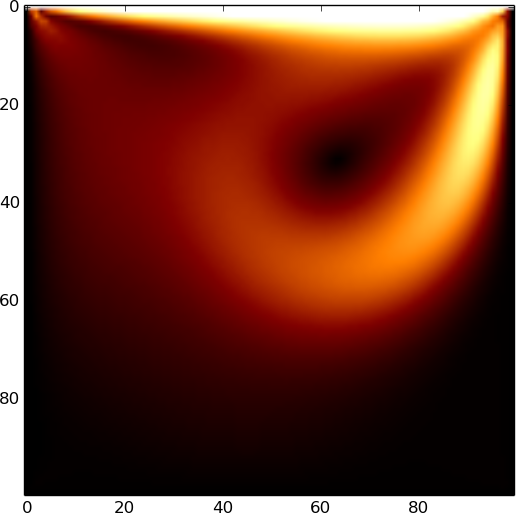
\includegraphics[width=0.8\linewidth]{../figures/ldc_re500_vel2_0019_trim.png} % chktex 11
  \caption{Velocity magnitude }
\end{subfigure}%
\begin{subfigure}{.5\textwidth}
\label{fig: density SRT}
  \centering
  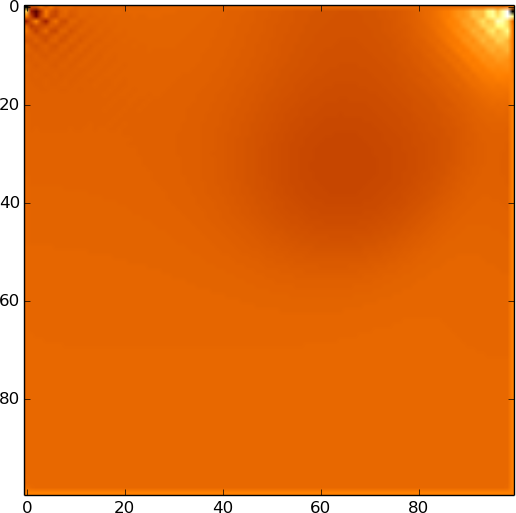
\includegraphics[width=0.8\linewidth]{../figures/ldc_re500_rho2_0019_trim.png} % chktex 11
  \caption{Density fluctuations}
\end{subfigure}
\caption{Simulation of a lid driven cavity with SRT LBM at $Re=500$. Especially in the density field, we can see the checkerboard pattern of upcoming instabilities.}
\label{fig: spurious modes SRT}
\end{figure}

Intuitively, we can describe \gls{srt} as a scheme, where all non-conserved quantities which can be computed from the \glspl{pdf}, are relaxed at the same rate.
Hence we impose, that all events that happen in the fluid occur at the same rate, which is certainly not true.

This was noticed soon after its publication and apparently the remedy was found by d'Humiéres,~\cite{d1994generalized}, who proposed to change from the space of particle distributions to the space of moments and relax linear combinations of those independently.
This was the birth of the \gls{mrt} schemes.
Unfortunately, even today there is no consent about how to choose all the relaxation parameters in an optimal way.
Although, when chosen right, the accuracy and stability can improve greatly in contrast to SRT, allowing simulations of $Re$ in the low thousands, c.f.~\cite{d2002multiple}. Still, this does not nearly cover the regions we see in Table~\ref{table: reynolds numbers}.

The source of these problems can be interpreted as the violation of \gls{galInv}, as deduced in~\cite{geier2006cascaded}. Consequently, the authors choose the space of central moments for the relaxation, as they are centered around the first moment, i.e.\ the velocity times density.
This method is capable of simulating \gls{re} way above the ones, \gls{mrt} was capable of and is used in industrial grade \gls{lbm} solvers, like \href{http://www.xflowcfd.com/technology/view/cfd}{xFlow}.

Nevertheless, we will introduce yet another set of characteristic variables in the next Section and explain the physical reasoning behind choosing them.
